
\documentclass[12pt,letterpaper]{article}
\usepackage{graphicx}
\graphicspath{{images/}}
\begin{document}
	
	\title{COLLEGE OF COMPUTING AND INFORMATION SCIENCES\\ DEPARTMENT OF COMPUTER SCIENCE\\ SCHOOL OF COMPUTING AND INFORMATICS TECHNOLOGY\\}
	\maketitle
	
	\title{NAME:	         OKIRING PAUL \space-214016765  - 14/U/13973/EVE   
		\maketitle
		\\
		\\
		\begin{center}
			\title {\textbf{REPORT}}
		\end{center}
		\title{\textbf{IS MONEY A MAJOR NECESSITY IN A RELATIONSHIP AMONG THE YOUTH}}
		\maketitle
		
		\section{INTRODUCTION}
		Relationships (or even finding the right person to have a relationship with) can be pretty complicated. To make it work, you have to have something in common, you need to be able to communicate, and there must be some special chemistry going on. A romantic might tell you that love and money shouldn’t have anything to do with each other, but while money won’t make a relationship, it can break them. This issue has been on for a long time on whether money really matters in a relationship among the youth. Is it the no.1 most priority? Is it the only thing that can sustain a relationship? We are yet to find out the answer
		
		\section{PROBLEM STATEMENT}
		Money is so strong to the extent it can break that special bond between you and your love partner. Some relationships go south (break) when it comes to money matters. Finding out whether money is a top priority will help make awareness and reduce on rampant breakups.  Collecting this data will help us find out whether money really is a major necessity. This will in return help to improve on the health of the various relationships happening out there.
		
		\section{PURPOSE OF STUDY}
		The purpose of this study is to help us understand whether money is a major necessity in relationships among the youth
		\section{MAIN OBJECTIVE}
		To find out whether money is a major necessity in relationships among the youth.
		\subsection{OBJECTIVES}
		\begin{enumerate}
			
			\item To find whether boys and girls from a rich family status take money as a major necessity in relationships\\
			\item To find whether boys and girls from a poor family status take money as a major necessity in relationships\\
			\item To find whether boys and girls from a well off family status take money as a major necessity in relationships\\
			
		\end{enumerate}
		
		
		\section{DATA ANALYSIS}
		\subsection{table 1}
		
		
		
		\begin{tabular}{ |p{1cm}||p{2cm}|p{2cm}|p{1cm}|p{2cm}|p{1cm}  }
			\hline
			\multicolumn{6}{|c|}{GIRLS} \\
			\hline
			Family Status & Consider Money(CM)&Dont Consider Money(DCM) &Total& percent of CM& Percent of DCM\\
			\hline
			Rich   & 1    &4&  5&20&80\\\\
			Poor&6&1&7&85.71&14.28\\\\
			Well Off &1&2&3&33.33&66.667\\\\
			\hline
		\end{tabular}
		
		\subsection{table 2}
		
		
		\begin{tabular}{ |p{1cm}||p{2cm}|p{2cm}|p{1cm}|p{2cm}|p{1cm}  }
			\hline
			\multicolumn{6}{|c|}{BOYS} \\
			\hline
			Family Status & Consider Money(CM)&Dont Consider Money(DCM) &Total& percent of CM& Percent of DCM\\
			\hline
			Rich   & 1   &3&  4&25&75\\\\
			Poor&1&4&5&20&80\\\\
			Well Off &1&5&6&16.67&83.33\\\\
			\hline
		\end{tabular}
		
		\section{Abbreviations}
		CM -\space Consider Money
		\\
		DCM - \space Don't Consider Money
		\\
		percent - \space percentage
		\section{SCREEN SHOTS OF APPLICATION}
		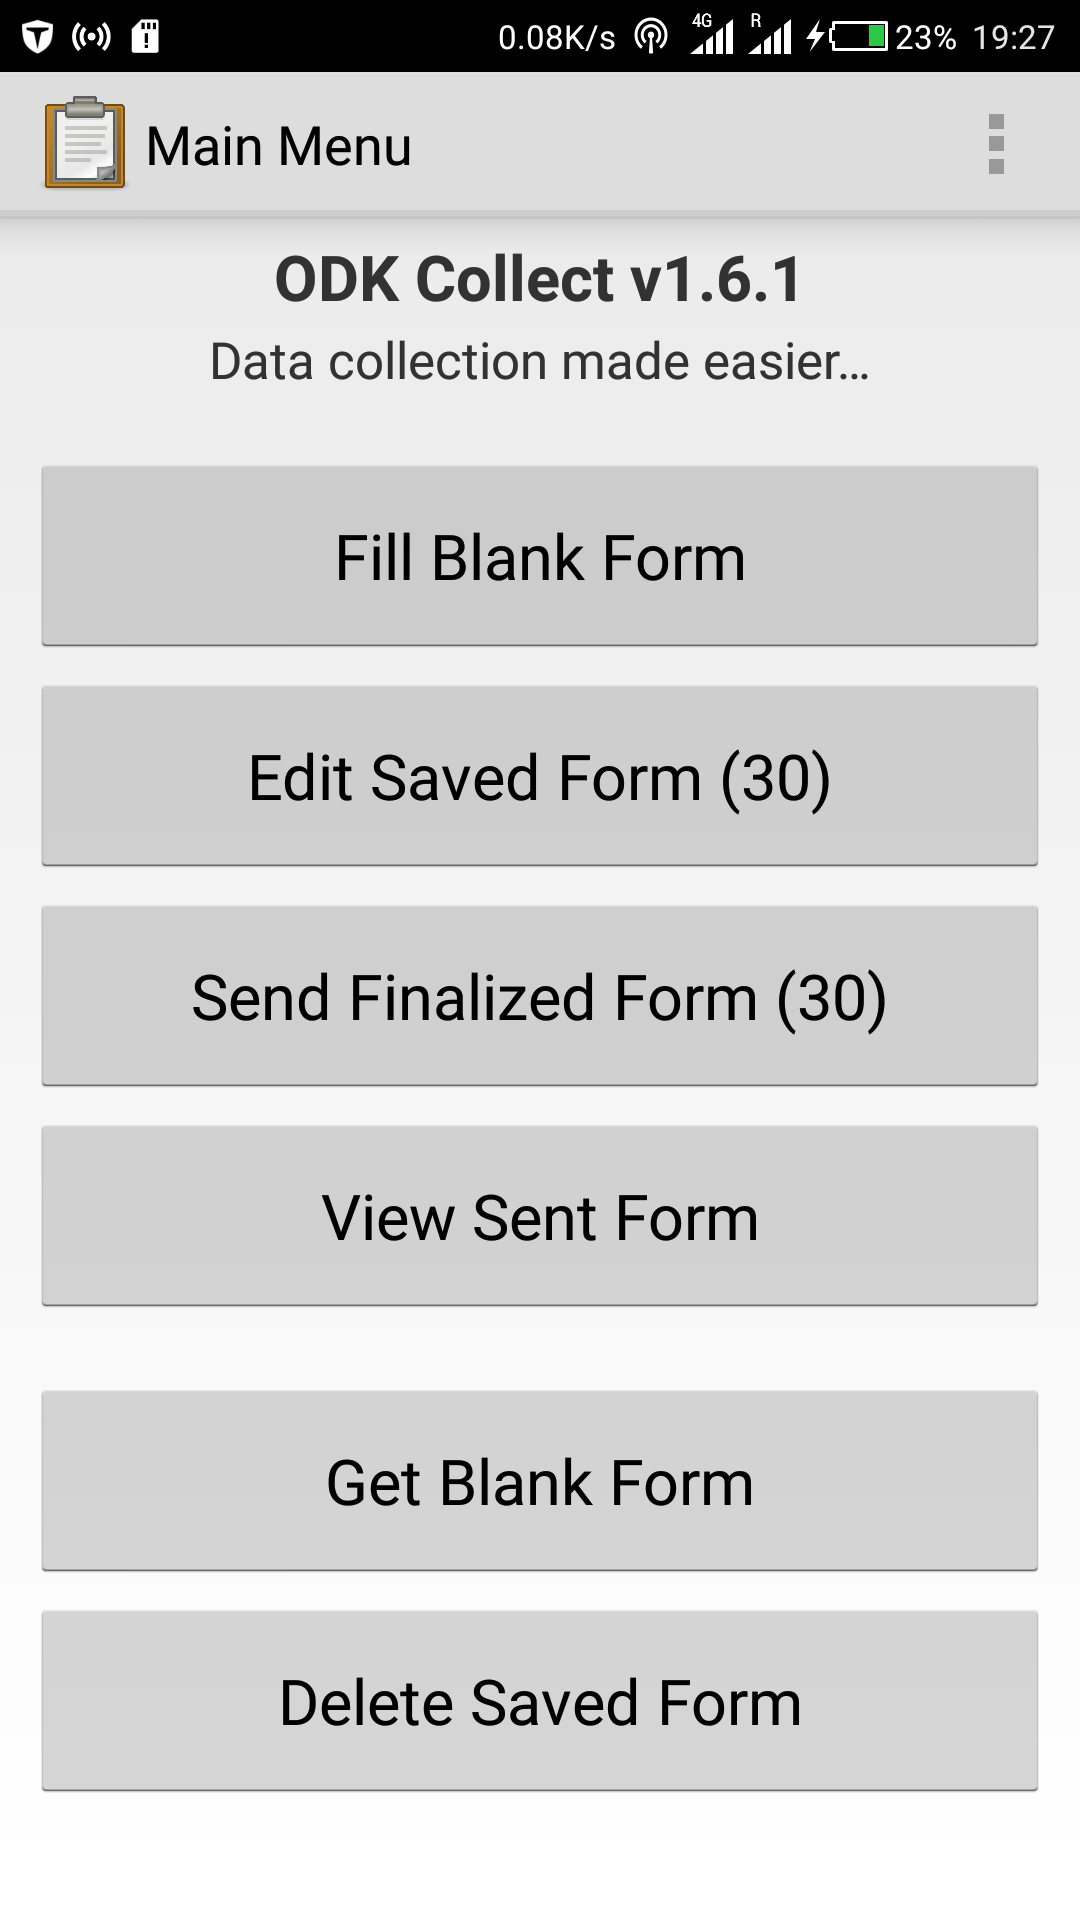
\includegraphics[scale=0.1]{cccc}
			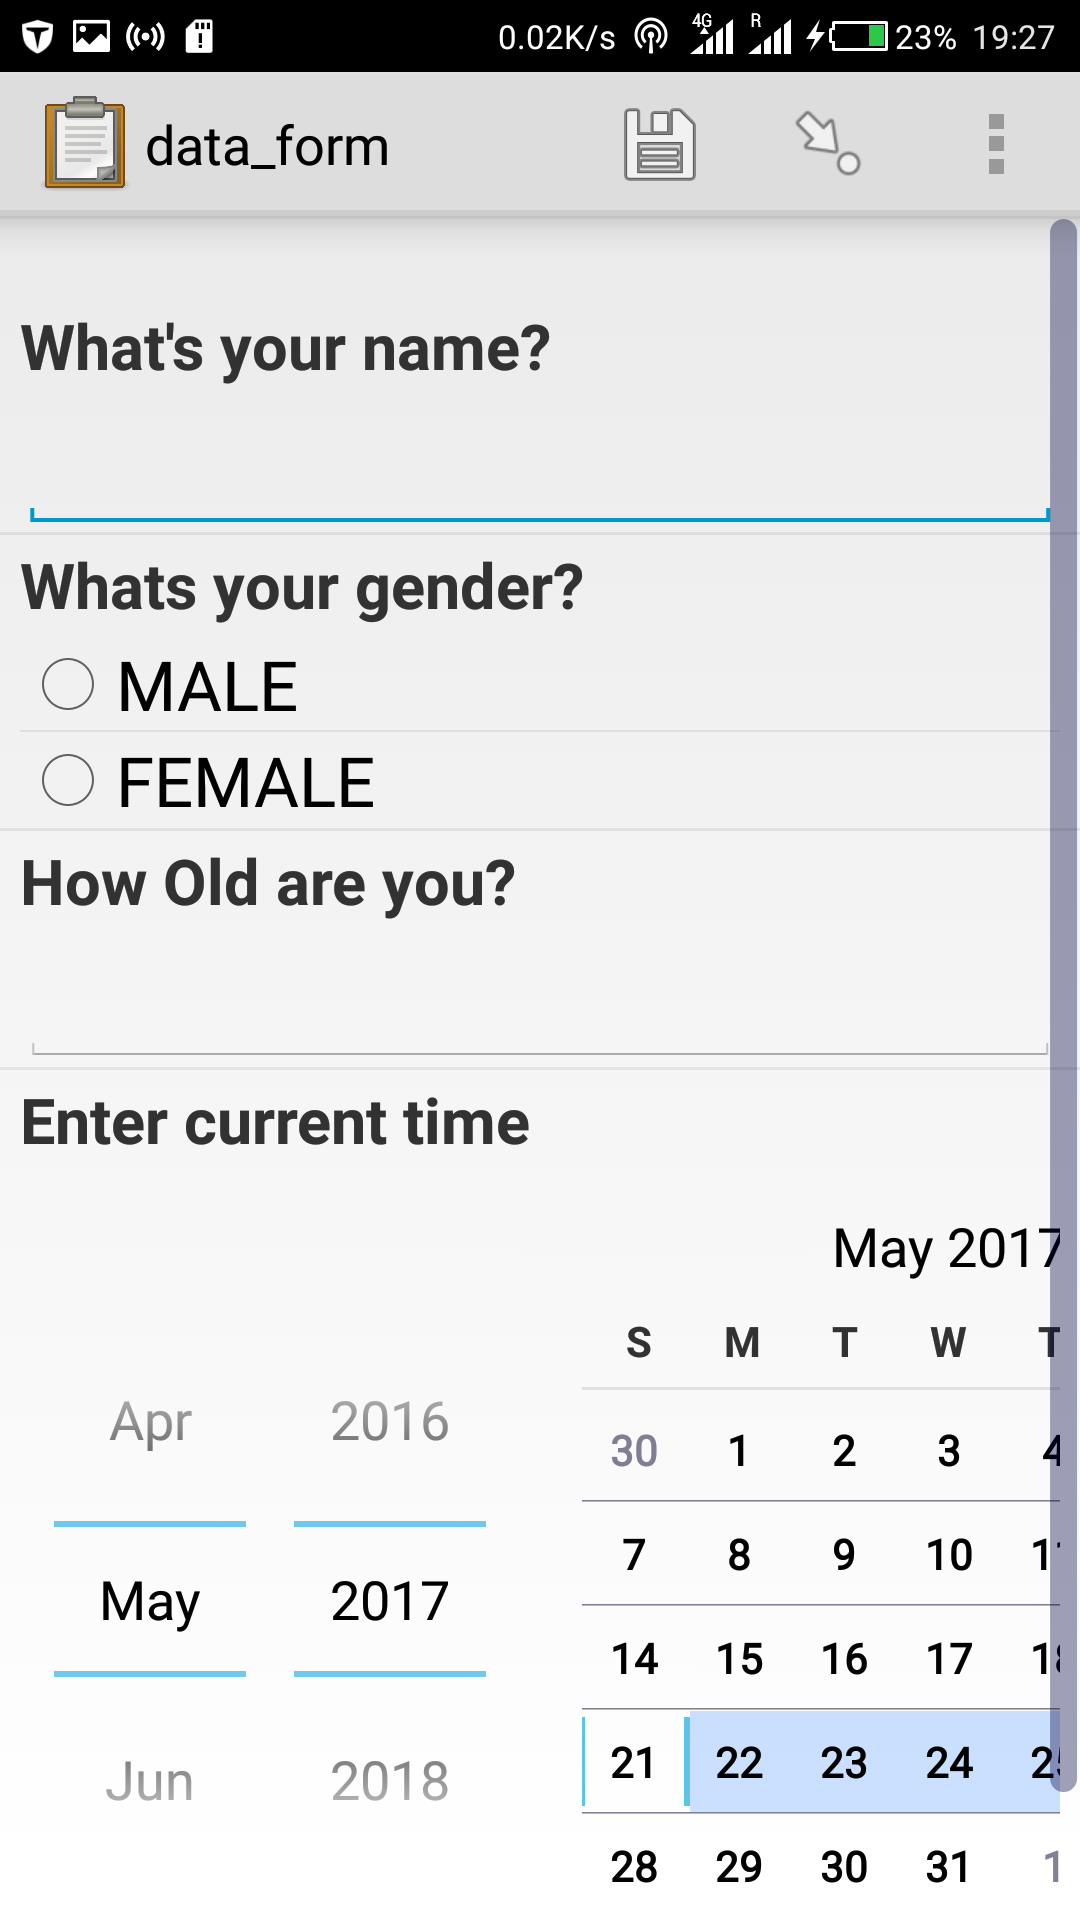
\includegraphics[scale=0.1]{paul1}
				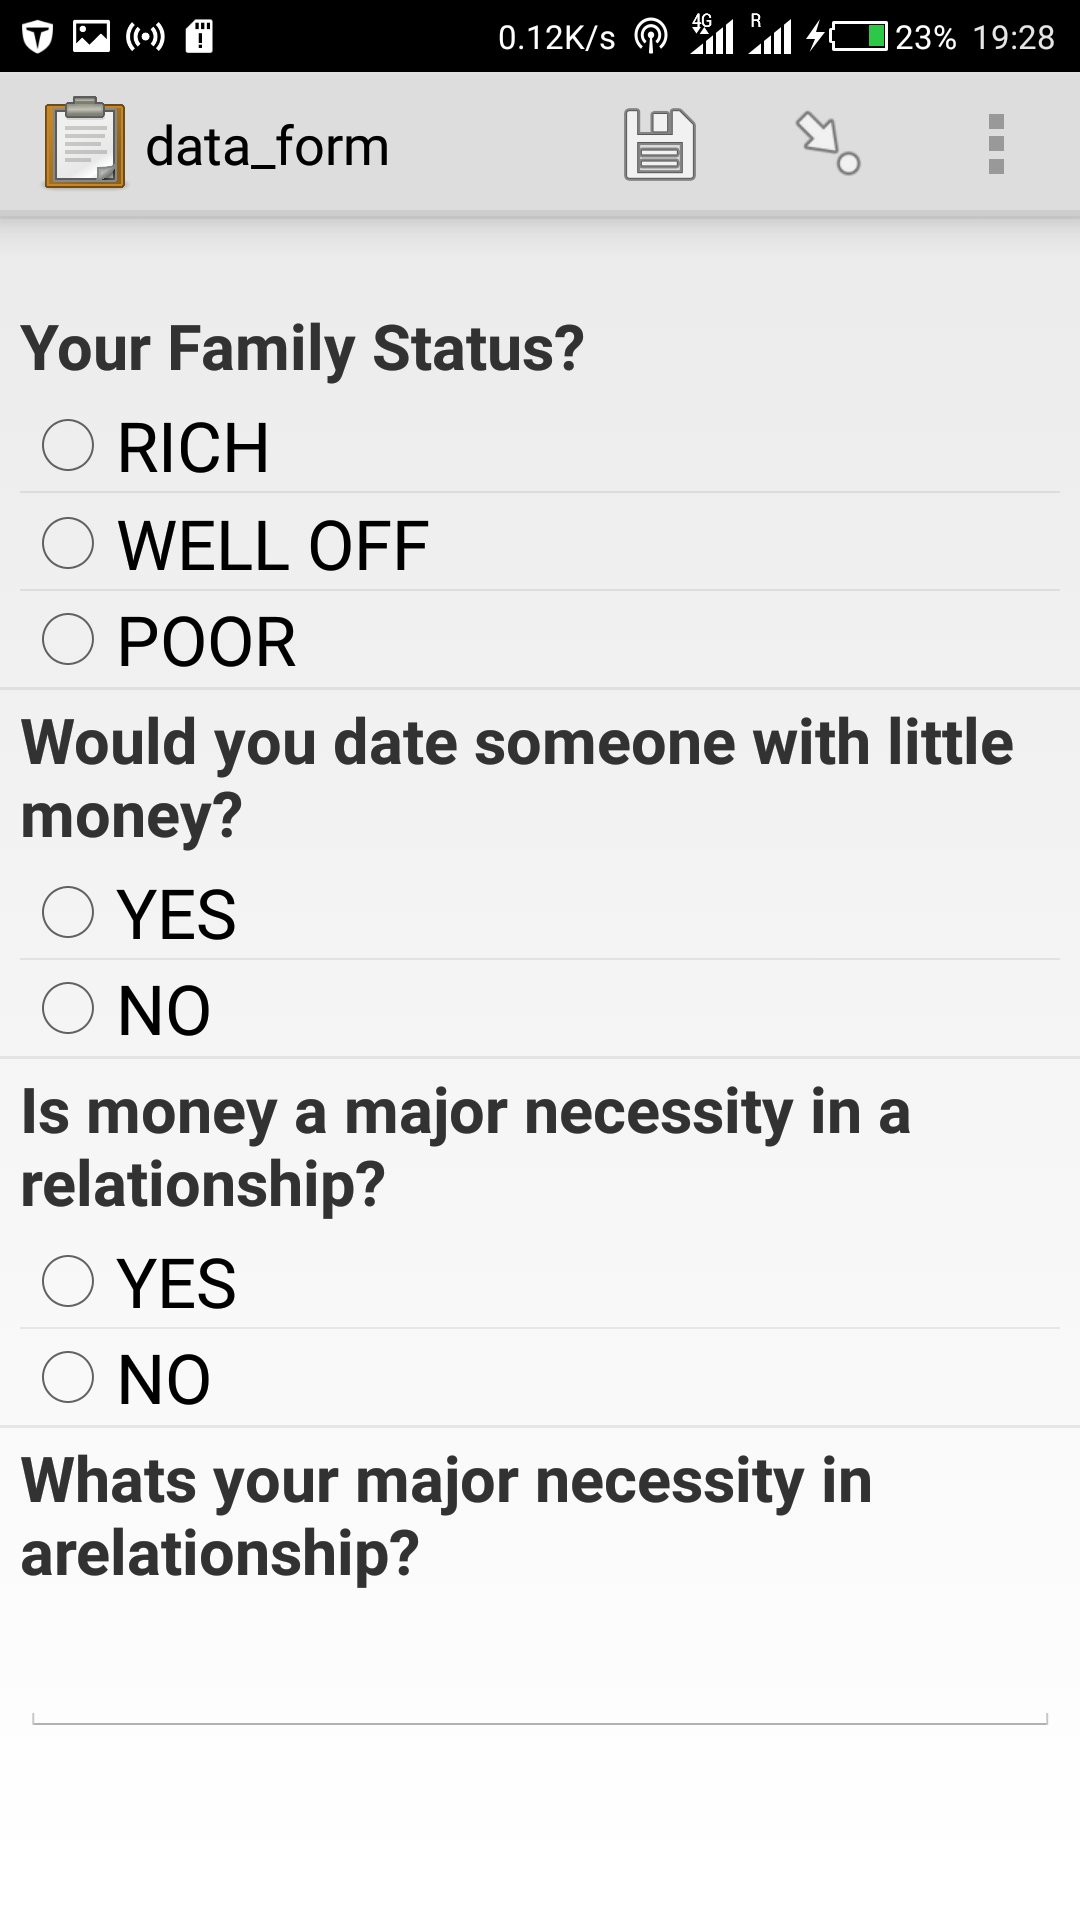
\includegraphics[scale=0.1]{paul2}
					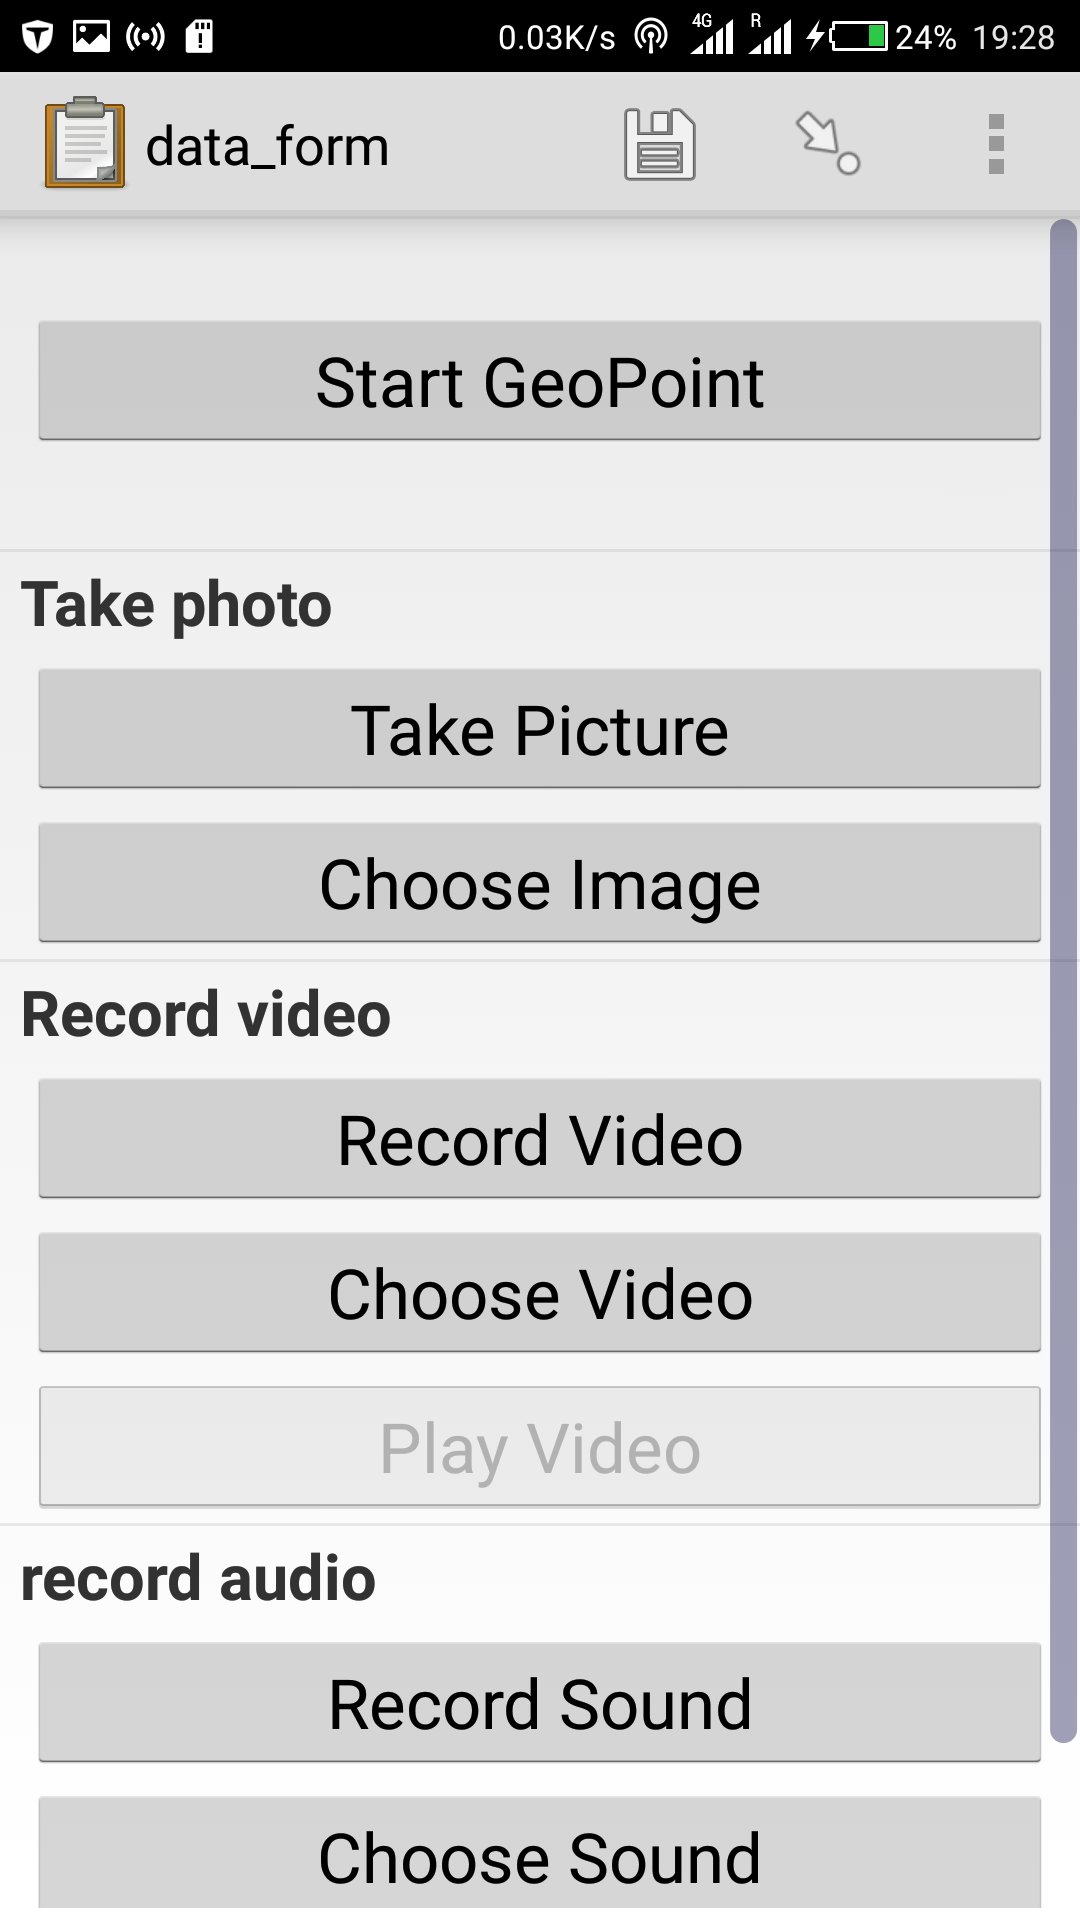
\includegraphics[scale=0.1]{paul3}
						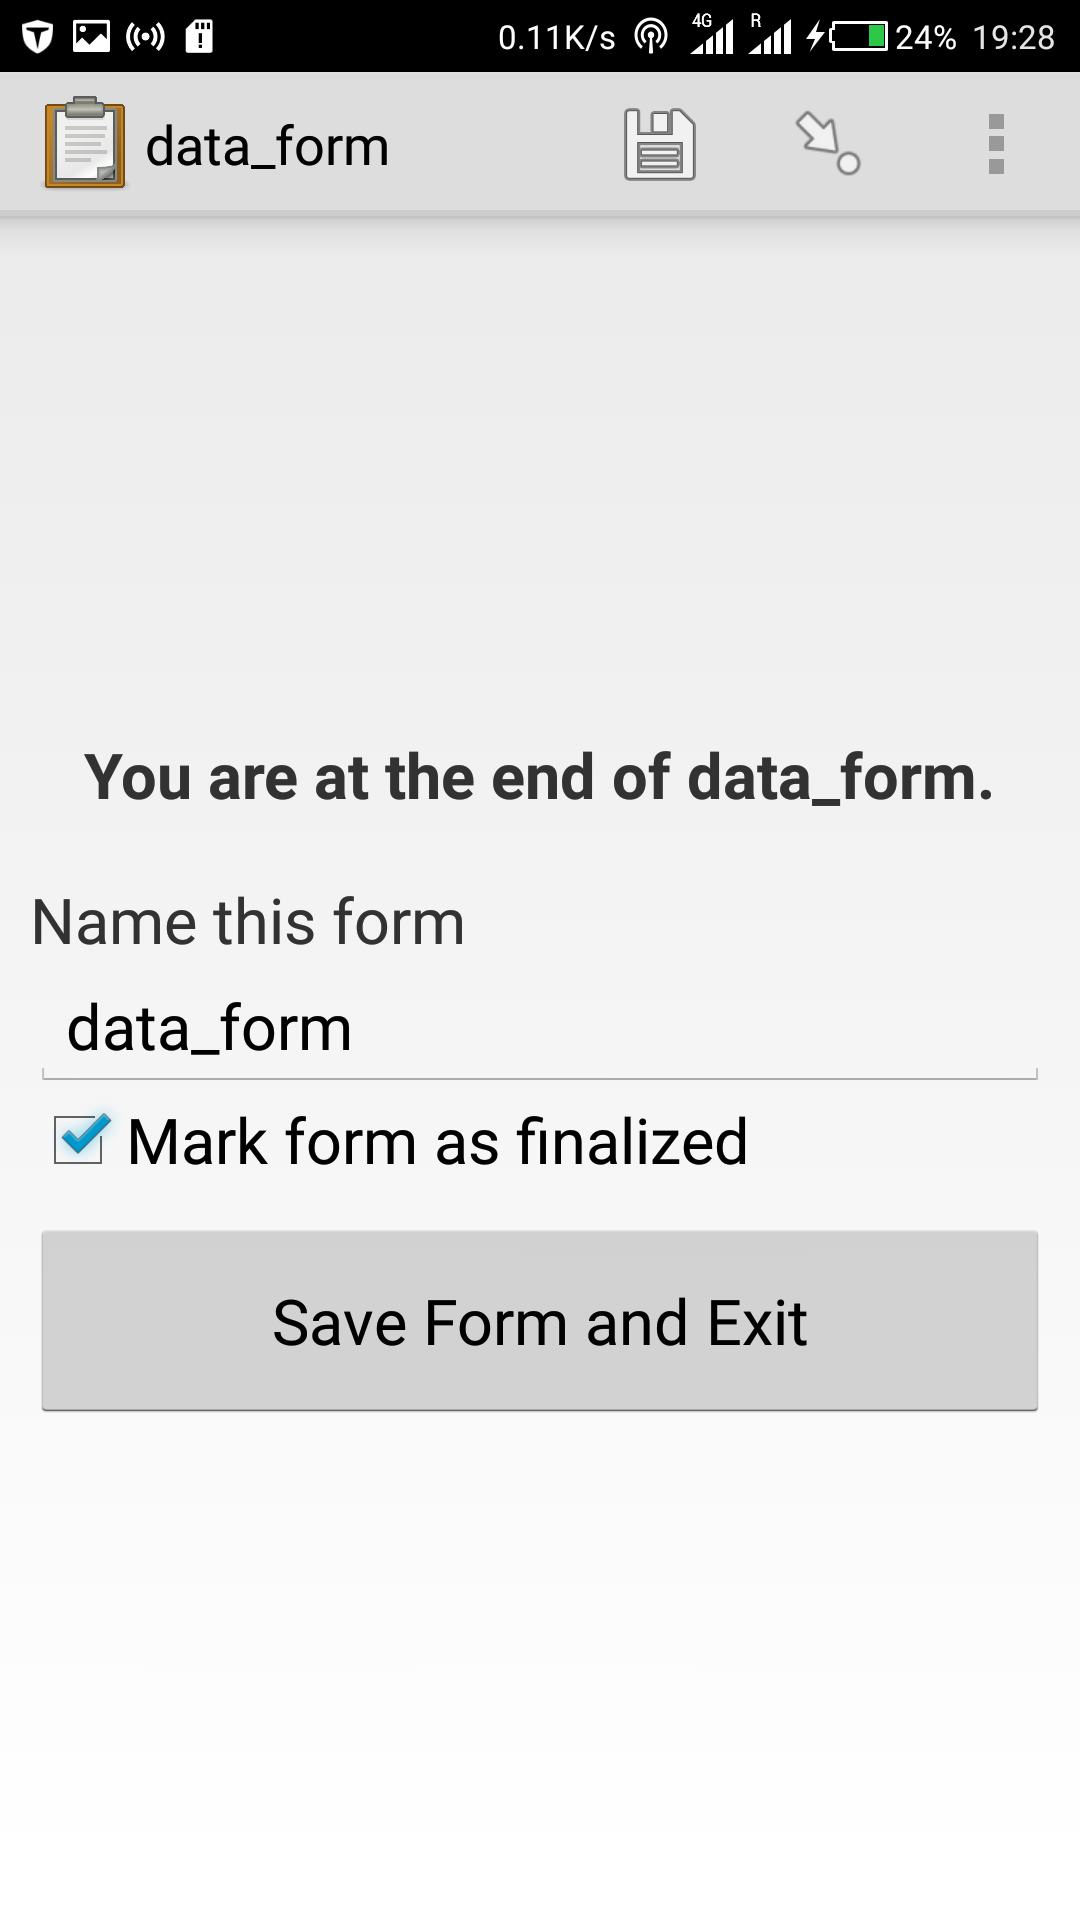
\includegraphics[scale=0.1]{paul4}
							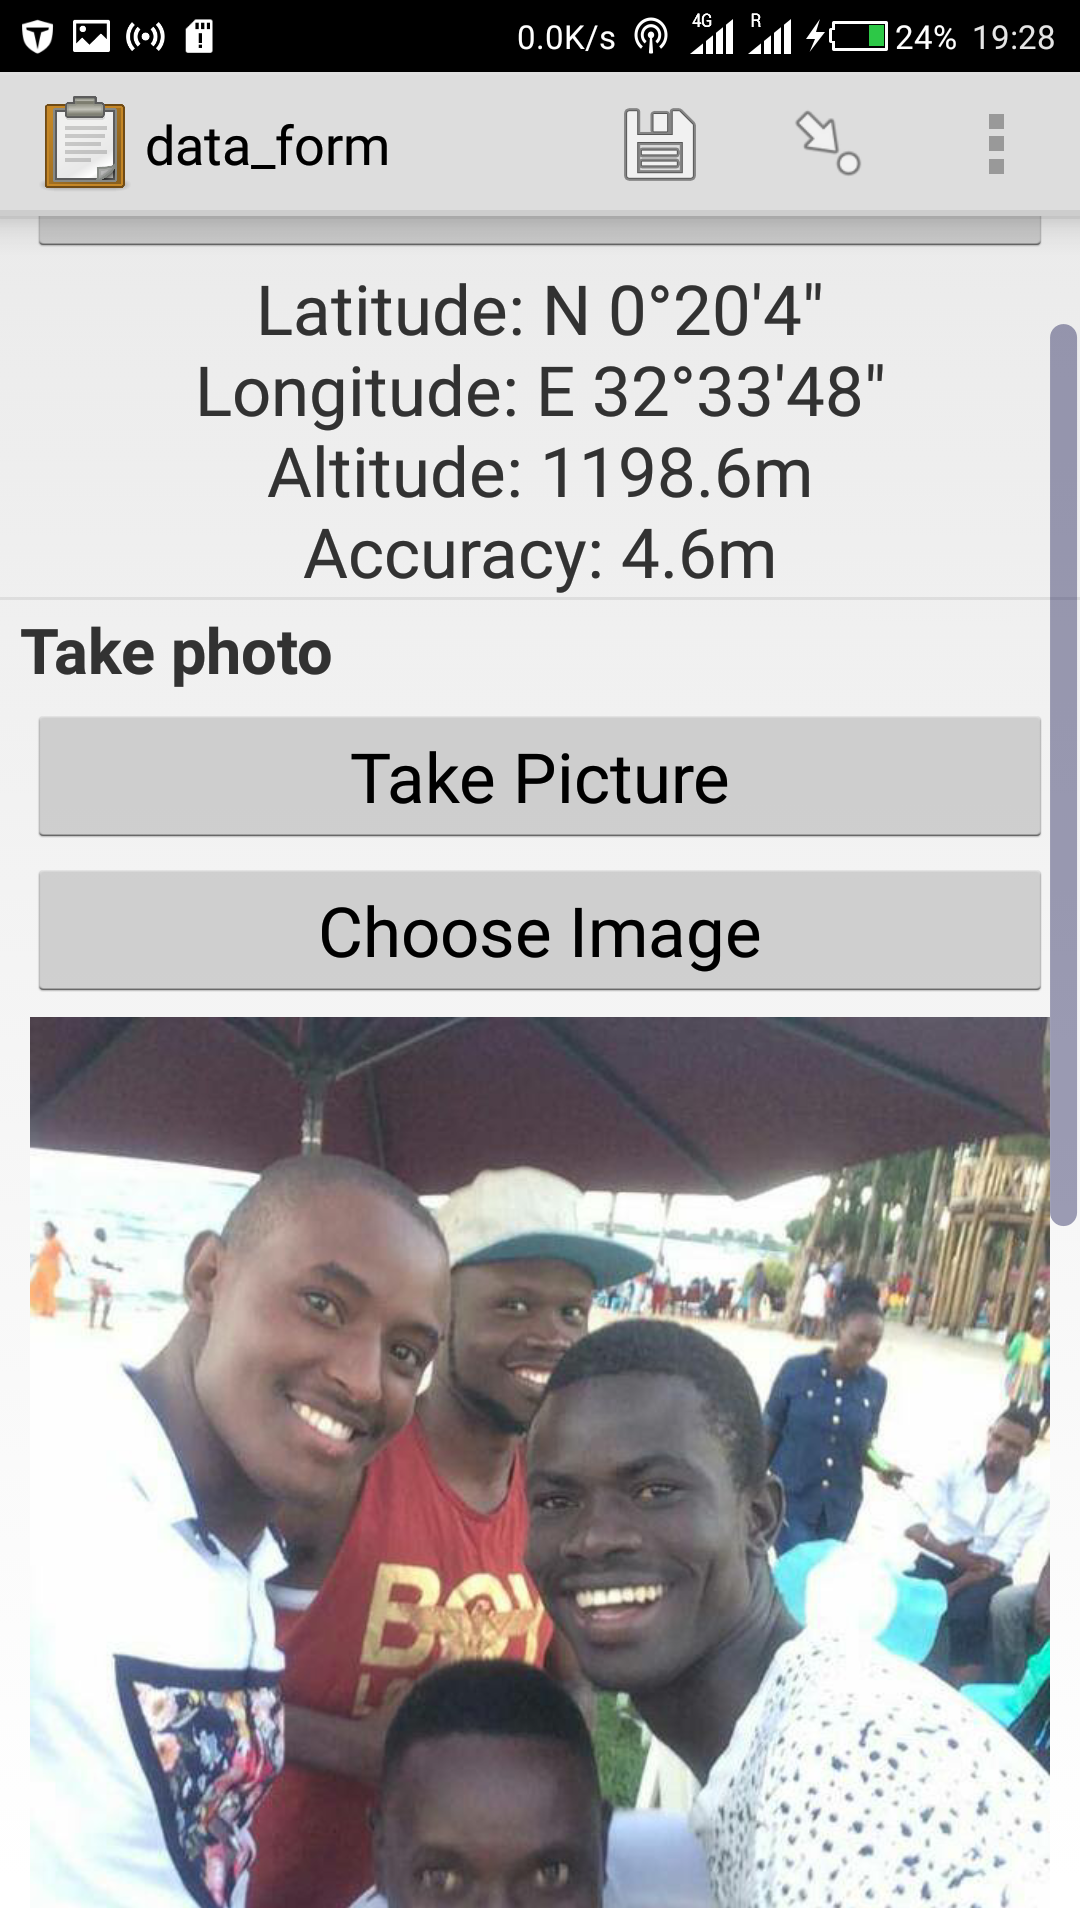
\includegraphics[scale=0.1]{paul5}
								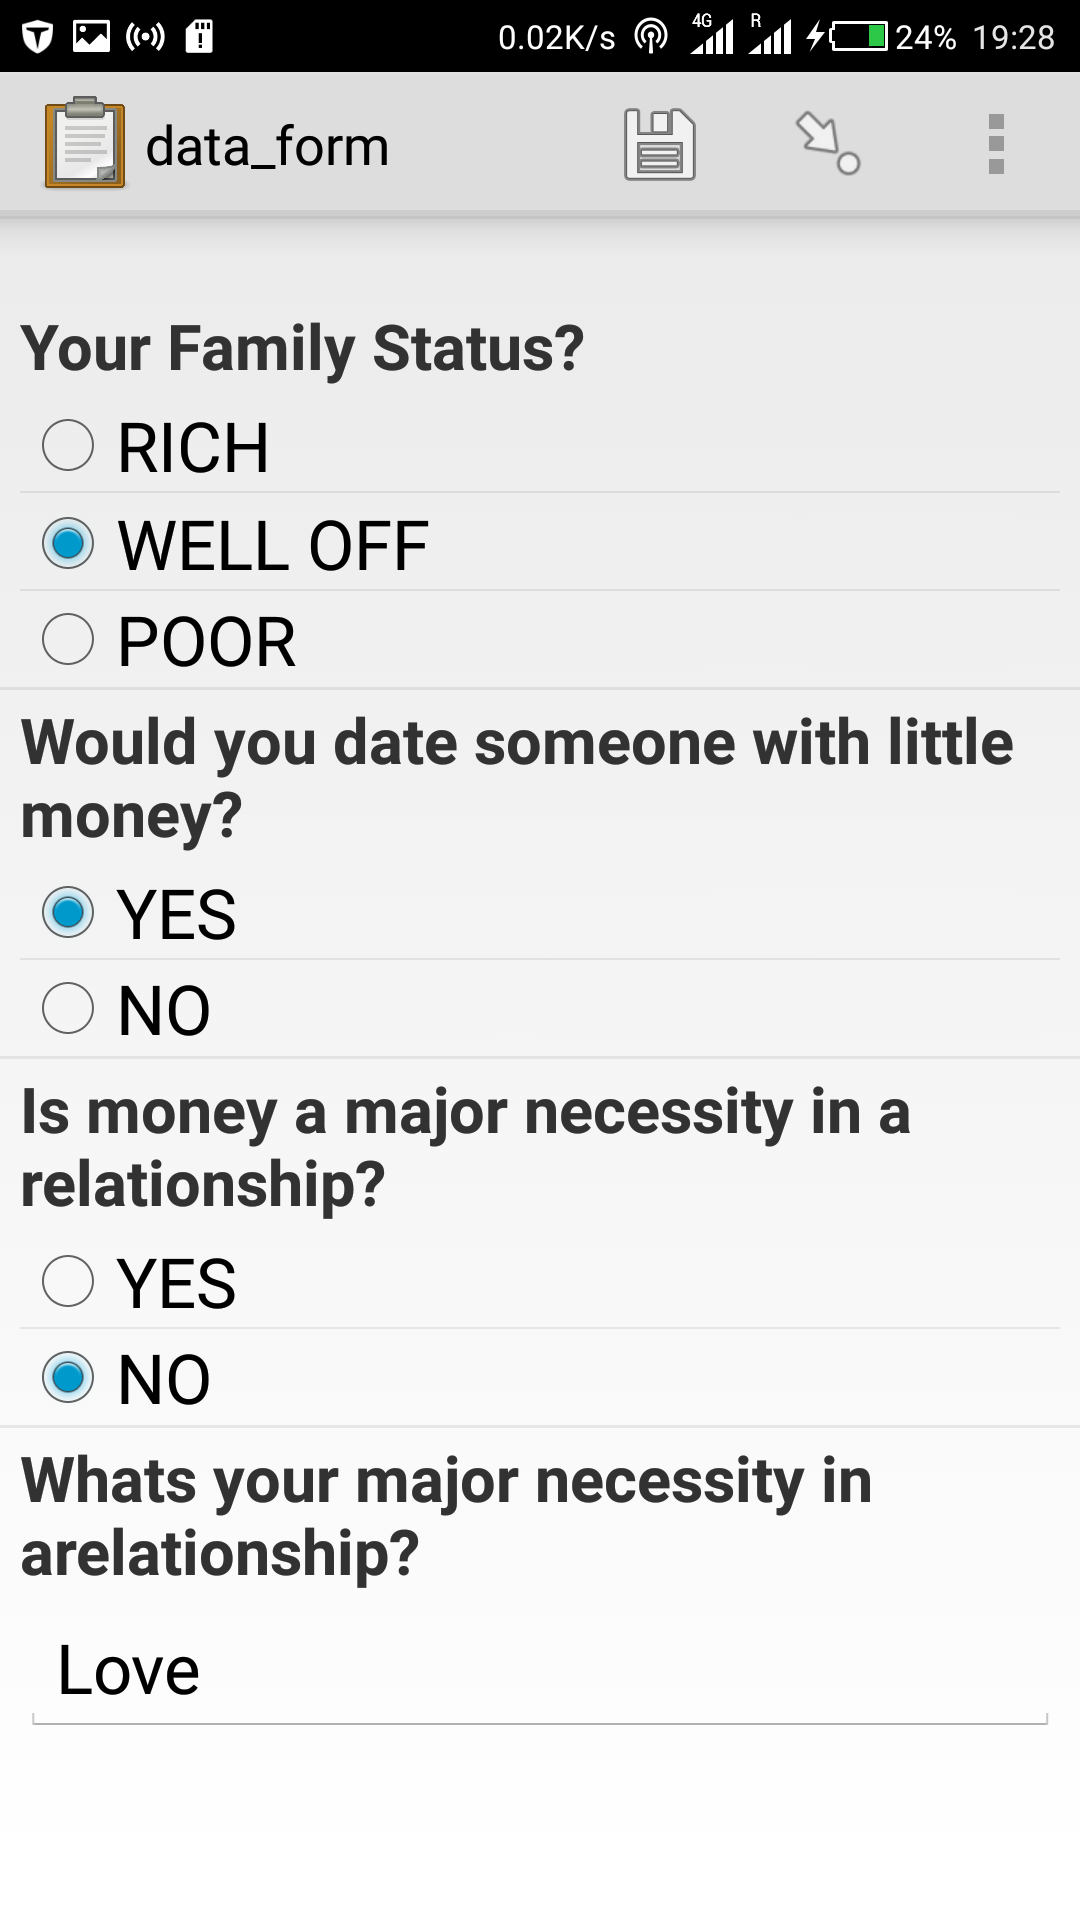
\includegraphics[scale=0.1]{paul6}
		
		
		
		\section{CONCLUSION}
		From the information i collected, its noticed that most girls with a poor family status consider money when it comes to relationships. Most take it as a major necessity. One of the reasons they gave me was that they need the money to buy commodities and since their families fail to provide, they look for other means to attain the money.most  Girls with a rich family status and those with a well off status don't take money as a major necessity in relationships.
		\\
		When it came to the boys, its noticed that most of them don't take money as a major necessity when it comes to relationships. They are Neutral 
	
		
	\end{document} 